\documentclass[11pt]{article}
\usepackage[margin=1in]{geometry}
\usepackage[T1]{fontenc}
\usepackage{lmodern}
\usepackage{amsmath}
\usepackage{booktabs}
\usepackage{graphicx}
\usepackage{caption}
\usepackage{setspace}
\usepackage[none]{hyphenat}        % no automatic word breaking with hyphens
\usepackage[round]{natbib}
\usepackage[hidelinks]{hyperref}
\graphicspath{{../results/figures/}}
\captionsetup{font=small, labelfont=bf, justification=raggedright, singlelinecheck=false}
\setstretch{1.25}
\sloppy
\newcommand{\NFirms}{519}
\newcommand{\NDelisted}{71}
\newcommand{\NStockMonths}{81{,}118}
\newcommand{\FirstMonth}{October 1998}
\newcommand{\LastMonth}{October 2026}
\newcommand{\NMonths}{335}
\newcommand{\SlopeMean}{1.00}
\newcommand{\SlopePos}{99.7}
\newcommand{\LSew}{1.46}
\newcommand{\LSewT}{4.70}
\newcommand{\LSvw}{0.75}
\newcommand{\LSvwT}{1.83}
\newcommand{\LSewAnn}{17.6}
\newcommand{\VALew}{1.67}
\newcommand{\VALewT}{4.54}
\newcommand{\VALvw}{1.32}
\newcommand{\VALvwT}{3.30}
\newcommand{\FFew}{0.90}
\newcommand{\FFewT}{3.73}
\newcommand{\FFvw}{\ensuremath{-}0.02}
\newcommand{\FFvwT}{\ensuremath{-}0.06}
\newcommand{\HMLew}{0.62}
\newcommand{\MicroFF}{0.31}
\newcommand{\MicroFFT}{1.31}
\newcommand{\MicroLS}{0.91}
\newcommand{\MicroLST}{2.96}
\newcommand{\TEXew}{1.42}
\newcommand{\TEXewT}{3.58}
\newcommand{\TEXff}{0.97}
\newcommand{\TEXffT}{2.57}
\newcommand{\BANKew}{0.55}
\newcommand{\BANKewT}{1.44}
\newcommand{\CEMew}{0.86}
\newcommand{\CEMewT}{1.72}
\newcommand{\ICmkt}{0.021}
\newcommand{\ICmktT}{2.86}
\newcommand{\Kew}{0.34}
\newcommand{\KewT}{1.09}
\newcommand{\Kvwff}{1.12}
\newcommand{\KvwffT}{2.96}
\newcommand{\ROEvwff}{1.21}
\newcommand{\ROEvwffT}{3.09}
\newcommand{\Turn}{34}
\newcommand{\HitM}{50.1}
\newcommand{\BaseM}{49.6}
\newcommand{\HitA}{51.5}
\newcommand{\BaseA}{49.0}
\newcommand{\HitAT}{2.44}
\newcommand{\NetHundred}{0.79}
\newcommand{\NetHundredT}{2.57}
\newcommand{\MktDef}{the value weighted return of the universe in excess of the three month Treasury bill yield}
\newcommand{\QoneEW}{2.16}
\newcommand{\QfiveEW}{3.63}
\newcommand{\TopEx}{0.93}
\newcommand{\TopExT}{4.80}
\newcommand{\FMfourResid}{0.21}
\newcommand{\FMfourResidT}{1.18}
\newcommand{\FMfourVal}{0.19}
\newcommand{\FMfourValT}{0.91}
\newcommand{\FMthreeROE}{0.09}
\newcommand{\FMthreeROET}{0.81}


\title{\textbf{Is the P/B ROE Model More Than Value?\\Evidence from the Pakistan Stock Exchange}}
\author{Ahmed Tallal Bajwa\thanks{Columbia Business School, MS in Financial Economics. Email: ab6333@columbia.edu.
This paper extends the author's undergraduate senior project at the Lahore University of Management Sciences.
Data: Compustat Global through Wharton Research Data Services; Treasury bill yields from the State Bank of Pakistan. All code is in the replication folder
that accompanies the paper.}}
\date{November 2026}

\begin{document}
\maketitle

\begin{abstract}
\noindent The P/B ROE model values a stock by its return on equity: firms that earn more on their book
equity should trade at higher price to book ratios, and a firm priced below that relation should
earn higher returns as the gap closes. I test the model on the Pakistan Stock Exchange using every
listed firm in Compustat Global, including \NDelisted{} firms that later delisted, from \FirstMonth{}
to \LastMonth{}. Accounting data enter only after they become public. The cross sectional relation
between ln(P/B) and ROE is strong and stable, and a portfolio long the stocks furthest below the
line and short those furthest above it earns \LSew{}\% a month equally weighted ($t = \LSewT{}$).
Three findings qualify this result. First, a plain low P/B sort earns as much, and in Fama and
MacBeth regressions ROE adds no information beyond P/B. Second, the return survives a three factor
adjustment only among equally weighted portfolios and disappears once microcaps are excluded.
Third, among the three largest sectors the model works within textiles but not within banks or
cement. Measured as a hit rate, the model is right only slightly more often than a classifier that
guesses with the same proportions. On the PSX the P/B ROE model is best read as a value strategy concentrated
in small, thinly traded stocks.
\end{abstract}

\section{Introduction}

Price to book ratios differ a great deal across firms. The P/B ROE model, set out by
\citet{wilcox1984} and revisited by \citet{wilcoxphilips2005}, explains much of that dispersion with
one variable: profitability. A firm that earns a high return on equity should be worth a multiple of
its book value, and a firm that earns less than its cost of capital should trade below book. Fitting
this relation across firms gives each stock an expected P/B; a stock priced below that expectation is
cheap given its profitability, and the model predicts that it will outperform as its price converges.

The model is popular with practitioners because it is simple and because it ties a valuation
multiple to a fundamental that analysts already forecast. It is also an appealing tool for emerging
markets, where analyst coverage is thin and mispricing is plausibly larger. This paper asks whether
the model earns abnormal returns on the Pakistan Stock Exchange (PSX), and whether whatever it earns
is new information or a restatement of the value premium.

Answering the question well requires attention to four problems that are easy to overlook in a
small market. The first is survivorship: a sample built from firms that are still listed today
excludes the firms that failed, which are disproportionately the cheap ones. The second is timing:
annual reports appear months after the fiscal year ends, and Pakistani firms use different fiscal
years (banks close in December, most industrial firms in June). The third is the benchmark: a hit
rate above 50\% is not evidence of skill when the share of stocks labelled cheap and the share that
outperform are both far from one half. The fourth is risk: a stock that is cheap relative to its ROE
is also usually cheap in absolute terms, so its returns must be compared with those of plain value.

I address each problem directly. The sample is every Pakistani firm in Compustat Global, active and
inactive, which gives \NFirms{} firms and \NStockMonths{} firm months between \FirstMonth{} and
\LastMonth{}. Fundamentals are used only four months after the fiscal year end. The P/B ROE line is
estimated afresh each month across firms, so the residual measures relative mispricing on that date
rather than the level of the market. Returns include dividends and are tested with long short
portfolios, Newey and West $t$ statistics, Fama and MacBeth regressions, factor models built from
the same universe, a hit rate compared with its chance rate, and a range of robustness checks.

The results are mixed and, I think, informative. The P/B ROE relation itself is very strong: the
monthly cross sectional slope of ln(P/B) on ROE averages \SlopeMean{} and is positive in
\SlopePos\% of months. Stocks far below the line do earn more: the equally weighted long short
portfolio earns \LSew{}\% a month ($t = \LSewT{}$), and \FFew{}\% a month after a market, size and
value adjustment ($t = \FFewT{}$). But a plain low P/B sort earns \VALew{}\% a month, and once P/B
is controlled for, neither ROE nor the residual predicts returns. The value weighted portfolio earns
little after the factor adjustment, and dropping the smallest 30\% of stocks removes the alpha. The
only sector where the model clearly works within the sector is textiles.

The paper contributes in three ways. It provides, to my knowledge, the first survivorship free test
of the P/B ROE model on the PSX with point in time accounting data. It separates the model's return
into its value and profitability components, which shows that on the PSX the return comes almost
entirely from the value side. And it implements the forward looking two period version of the model
of \citet{wilcoxphilips2005} as an implied expected return, which behaves very differently from the
residual and loads on profitability rather than value.

The rest of the paper is organized as follows. Section~\ref{sec:model} sets out the model and the
hypotheses. Section~\ref{sec:data} describes the data, Section~\ref{sec:method} the tests, and
Section~\ref{sec:results} the results. Section~\ref{sec:discussion} discusses limitations and
Section~\ref{sec:conclusion} concludes.

\section{The P/B ROE model}\label{sec:model}

\subsection{From dividends to price to book}

Let a firm have book equity $B$, a constant return on equity $ROE$, a payout ratio $d$, and a cost
of equity $k$. With clean surplus accounting, earnings are $ROE \cdot B$, dividends are
$d \cdot ROE \cdot B$, and book equity grows at $g = (1-d)\,ROE$. The constant growth dividend model
then gives
\begin{equation}
\frac{P}{B} = \frac{d \cdot ROE}{k - g} = \frac{ROE - g}{k - g}.
\label{eq:gordon}
\end{equation}
A firm that earns exactly its cost of equity ($ROE = k$) trades at book, a firm with $ROE > k$
trades above book, and the premium grows with the gap and with growth. The same conclusion follows
from the residual income model of \citet{ohlson1995}, in which price equals book value plus the
present value of expected earnings in excess of the cost of equity.

\subsection{The empirical model}

Equation~(\ref{eq:gordon}) is nonlinear, and $k$ and $g$ are not observed. \citet{wilcox1984}
proposed a linear relation in logs that fits the cross section well:
\begin{equation}
\ln\!\left(\frac{P}{B}\right)_{i,t} = a_{s,t} + b_t\, ROE_{i,t} + e_{i,t},
\label{eq:wilcox}
\end{equation}
estimated across firms $i$ at date $t$. I allow a separate intercept $a_{s,t}$ for each sector $s$ so
that differences in risk and growth across industries do not enter the residual. The residual
$e_{i,t}$ is the model's measure of mispricing: a negative residual means the stock is cheap given
its profitability.

\subsection{The two period model}

\citet{wilcoxphilips2005} make the model forward looking. Suppose a firm earns $ROE$ on book equity
for $T$ years and pays no dividends in between. Its book grows at rate $ROE$, its price grows at the
expected return $k$, and so
\begin{equation}
\ln\!\left(\frac{P}{B}\right)_{0} = \ln\!\left(\frac{P}{B}\right)_{T} + (k - ROE)\,T.
\label{eq:twoperiod}
\end{equation}
If the fitted value from (\ref{eq:wilcox}) is taken as the P/B the firm will trade at by date $T$,
equation (\ref{eq:twoperiod}) can be solved for the expected return:
\begin{equation}
k_{i} = ROE_{i} - \frac{e_{i}}{T}.
\label{eq:implied}
\end{equation}
The implied return has two parts: the profitability the firm keeps earning, and the convergence of
its price to the line, spread over $T$ years. I set $T = 5$. The residual alone isolates the
convergence part; $k_i$ adds the profitability part.

\subsection{Hypotheses}

The model gives three testable predictions. \textbf{H1}: stocks with negative residuals earn higher
future returns than stocks with positive residuals. \textbf{H2}: the residual predicts returns beyond
what P/B alone predicts; otherwise the model adds nothing to a plain value strategy. \textbf{H3}: the
relation holds within sectors, where firms share business models and the linear fit should work best.

\section{Data}\label{sec:data}

\subsection{Sources and sample}

All data come from Compustat Global through WRDS. The universe is every company incorporated or
headquartered in Pakistan, active or inactive: 668 companies, of which 519 enter the final sample
after the filters below. Prices, shares outstanding, trading volume, adjustment factors and total
return factors come from the daily security file; book equity and earnings come from the annual
fundamentals file; the KSE100 index comes from the index file. The risk free rate is the monthly average of the
weighted average yield at the State Bank of Pakistan's 3 month Treasury bill auctions, available for
every month of the sample. For each firm I use its longest
running share class.

Monthly returns are computed from a total return index, so they include cash dividends. A return
is computed only between two consecutive month ends. Following the advice of \citet{inceporter2006}
for international data, monthly returns above 300\% are treated as data errors and set to missing;
this affects 50 of about 131,000 monthly returns.

\subsection{Variables and timing}

Book equity is common equity (\texttt{ceq}), or total shareholders' equity when common equity is
missing. ROE is income before extraordinary items divided by book equity at the start of the fiscal
year. Annual accounts are used from the end of the fourth month after the fiscal year end, which
matches the 120 days within which a listed company must hold its annual general meeting, and for at most fourteen months after that. A bank
with a December year end therefore enters at the end of April, and a textile firm with a June year
end at the end of October. Market capitalization is the month end price times shares outstanding,
and P/B is market capitalization over the latest public book equity, so P/B moves every month with
the price. Sectors are GICS sectors; banks, cement and textiles are identified by GICS codes, with
SIC codes as a fallback.

A stock enters the universe in a month if it has positive book equity, a public ROE, a price of at
least PKR 1, and trades on at least five days of the month. The last condition matters on the PSX,
where many listed firms trade rarely. Table~\ref{tab:sample} describes the sample.

\begin{table}[htbp]
\centering\small
\caption{Sample. Firms is the number of distinct firms that ever enter the universe; delisted is
the number of those firms that are inactive in Compustat today. Firms per month is the average
number in the universe. Medians are over all firm months. Size is market capitalization in millions
of rupees.}
\label{tab:sample}
\footnotesize
\begin{tabular}{lrrrrrr}
\toprule
Sample & Firms & Delisted & Firms per month & Median P/B & Median ROE & Median size \\
\midrule
All firms & 519 & 71 & 242 & 0.98 & 0.118 & 2,837 \\
Banks & 29 & 9 & 16 & 0.93 & 0.139 & 22,392 \\
Cement & 19 & 1 & 13 & 1.07 & 0.107 & 6,323 \\
Textiles & 109 & 15 & 39 & 0.48 & 0.078 & 910 \\
\bottomrule
\end{tabular}

\end{table}

The sample is thin in the early years (fewer than 80 firms a month before 2001) and broad from
2012 onward (between 237 and 406 firms a month). Textile firms are numerous, small and cheap, with a median P/B
of about half; banks are large and few.

\section{Method}\label{sec:method}

\paragraph{Signal.} At the end of every month I estimate equation~(\ref{eq:wilcox}) by OLS across all
firms in the universe, with ROE winsorized at the 1st and 99th percentiles of that month and an
intercept for each GICS sector. The cheapness score is the negative of the residual. For the sector
tests I estimate (\ref{eq:wilcox}) separately within banks, cement and textiles, with a single
intercept, whenever the sector has at least eight firms that month. The implied return $k_i$ follows
equation~(\ref{eq:implied}).

\paragraph{Portfolios.} Stocks are sorted into quintiles on each score at the end of month $t$ and
held over month $t+1$. Sector sorts use terciles, since a sector has only 16 to 49 firms a month.
The long short portfolio buys the cheapest group and sells the dearest. Portfolios are equally
weighted (EW) and value weighted (VW). As benchmarks I also sort on plain $-\ln(P/B)$ and on ROE alone.
Means are tested with Newey and West \citeyearpar{neweywest1987} $t$ statistics with six lags.

\paragraph{Risk adjustment.} I build market, size and value factors from the same universe, following
\citet{famafrench1993}: the market factor is \MktDef{}; SMB and HML come from six value weighted
portfolios formed on the median size and the 30th and 70th percentiles of book to market. Long
short returns are regressed on the market factor alone and on all three factors.

\paragraph{Cross sectional regressions.} To test H2 directly I run \citet{famamacbeth1973}
regressions of next month returns on standardized characteristics: the cheapness score, ln(B/P),
ROE, log size, and momentum (the return over months $t-11$ to $t-1$). Because the residual is a linear
combination of ln(P/B), ROE and sector dummies, the residual and ln(B/P) can be included together
but not alongside ROE.

\paragraph{Rank IC and hit rate.} The rank information coefficient is the monthly Spearman
correlation between the cheapness score and next month returns. The hit rate counts the share of
stocks for which ``cheap'' (negative residual) coincides with ``outperformed the cross sectional
average''. Its benchmark is not 50\%. If a share $p_u$ of stocks is labelled cheap and a share $p_o$
outperforms, a classifier that guesses at random with those proportions is right with probability
\begin{equation}
p_u\,p_o + (1-p_u)(1-p_o),
\label{eq:chance}
\end{equation}
which I call the chance rate. Because returns are skewed to the right, fewer than half of stocks beat
the average in a typical month, so the chance rate moves with the share labelled cheap. I report the
hit rate both monthly and for a 12 month horizon with formation at the end of each October.

\section{Results}\label{sec:results}

\subsection{The P/B ROE relation holds}

Figure~\ref{fig:scatter} shows the cross section at the end of October 2024. Profitable firms trade
at higher multiples, with a lot of dispersion around the line. Across all months the slope of
ln(P/B) on ROE averages \SlopeMean{} and is positive in \SlopePos\% of months. Figure~\ref{fig:slope}
shows that the slope varies over time: it is high for most of 2011 to 2019 and falls in the high inflation
years after 2021, when investors paid less for accounting profitability. The first part of the model,
that profitability explains valuation, is therefore well supported on the PSX.

\begin{figure}[htbp]
\centering
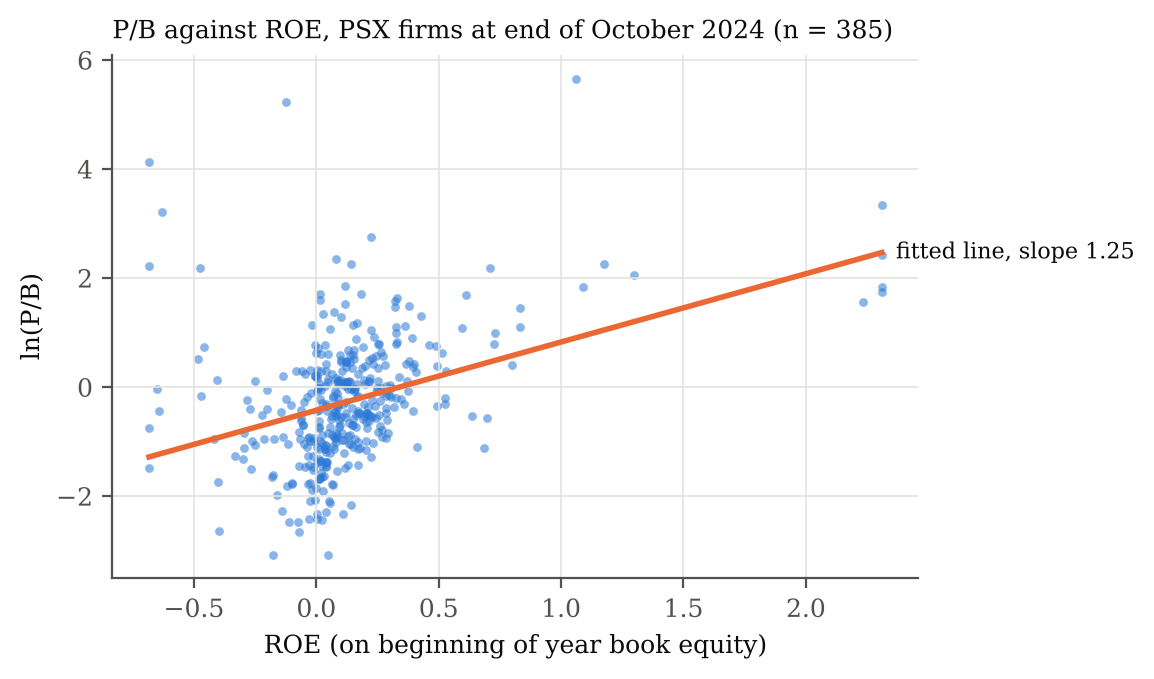
\includegraphics[width=0.72\textwidth]{fig1_pb_roe_scatter.png}
\caption{ln(P/B) against ROE for all firms in the universe at the end of October 2024, with a single
least squares line. The model's residual is the vertical distance from the line.}
\label{fig:scatter}
\end{figure}

\begin{figure}[htbp]
\centering
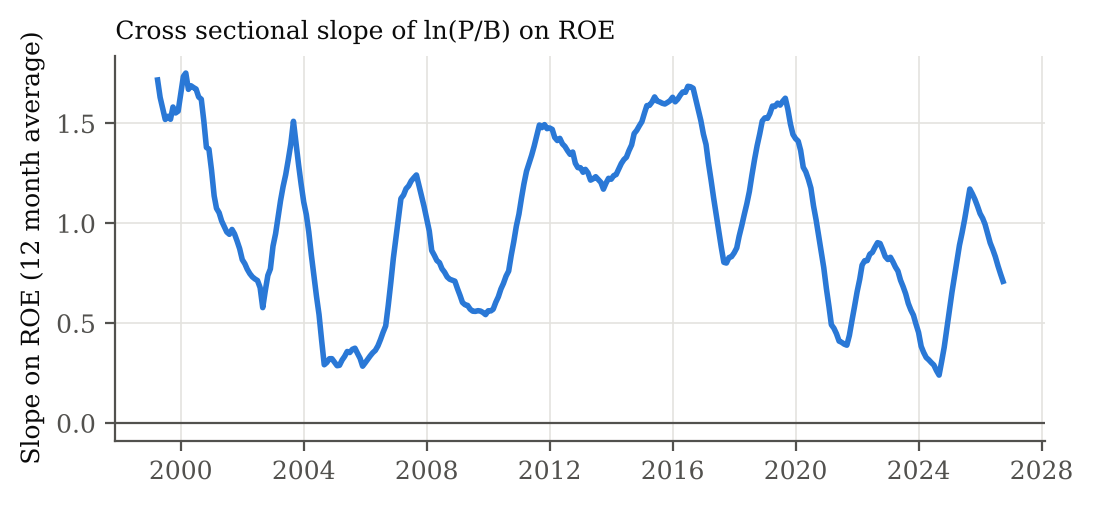
\includegraphics[width=0.85\textwidth]{fig4_slope_over_time.png}
\caption{Monthly slope of ln(P/B) on ROE from the whole market regression, 12 month moving average.}
\label{fig:slope}
\end{figure}

\subsection{Portfolio sorts}

Table~\ref{tab:quintiles} and Figure~\ref{fig:quintiles} report the returns of the quintiles. With
equal weights, returns rise from \QoneEW\% a month for the dearest quintile to \QfiveEW\% for the cheapest,
almost all of the spread coming from the cheapest quintile. The long short return is \LSew{}\% a
month ($t = \LSewT{}$), or \LSewAnn{}\% a year. With value weights the spread falls to \LSvw{}\%
($t = \LSvwT{}$): the effect is strongest in small stocks.

\begin{table}[htbp]
\centering\small
\caption{Mean monthly returns (\%) of quintile portfolios, with Newey and West $t$ statistics in
parentheses. Portfolios are formed each month on the P/B ROE residual (top two rows) or on plain
P/B (bottom two rows) and held for one month.}
\label{tab:quintiles}
\begin{tabular}{lrrrrrr}
\toprule
Sort & 1 (expensive) & 2 & 3 & 4 & 5 (cheap) & 5 minus 1 \\
\midrule
P/B ROE residual, EW & 2.16 & 2.42 & 2.60 & 2.68 & 3.63 & 1.46 \\
 & (4.97) & (5.21) & (5.47) & (5.86) & (6.59) & (4.70) \\
P/B ROE residual, VW & 1.65 & 2.17 & 2.48 & 2.35 & 2.40 & 0.75 \\
 & (4.23) & (4.91) & (5.29) & (4.65) & (4.19) & (1.83) \\
Plain low P/B, EW & 2.03 & 2.43 & 2.63 & 2.72 & 3.69 & 1.67 \\
 & (4.98) & (5.29) & (5.23) & (5.97) & (6.31) & (4.54) \\
Plain low P/B, VW & 1.54 & 2.12 & 2.34 & 2.46 & 2.86 & 1.32 \\
 & (4.42) & (4.62) & (4.67) & (4.93) & (4.93) & (3.30) \\
\bottomrule
\end{tabular}

\end{table}

\begin{figure}[htbp]
\centering
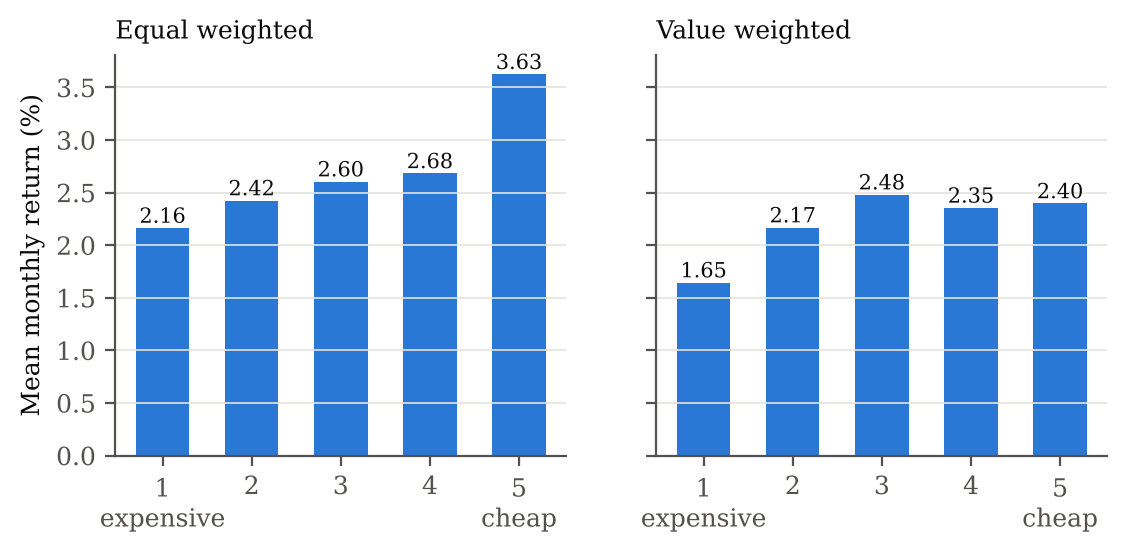
\includegraphics[width=0.85\textwidth]{fig2_quintile_returns.png}
\caption{Mean monthly returns of quintiles sorted on the P/B ROE residual.}
\label{fig:quintiles}
\end{figure}

The key comparison is with plain value. Sorting on P/B alone gives a long short return of
\VALew{}\% equally weighted and \VALvw{}\% value weighted, at least as much as the residual.
Figure~\ref{fig:cumulative} shows that the two strategies move together over the whole sample, with
plain value ahead in both weightings. Conditioning on ROE does not improve the value sort.

\begin{figure}[htbp]
\centering
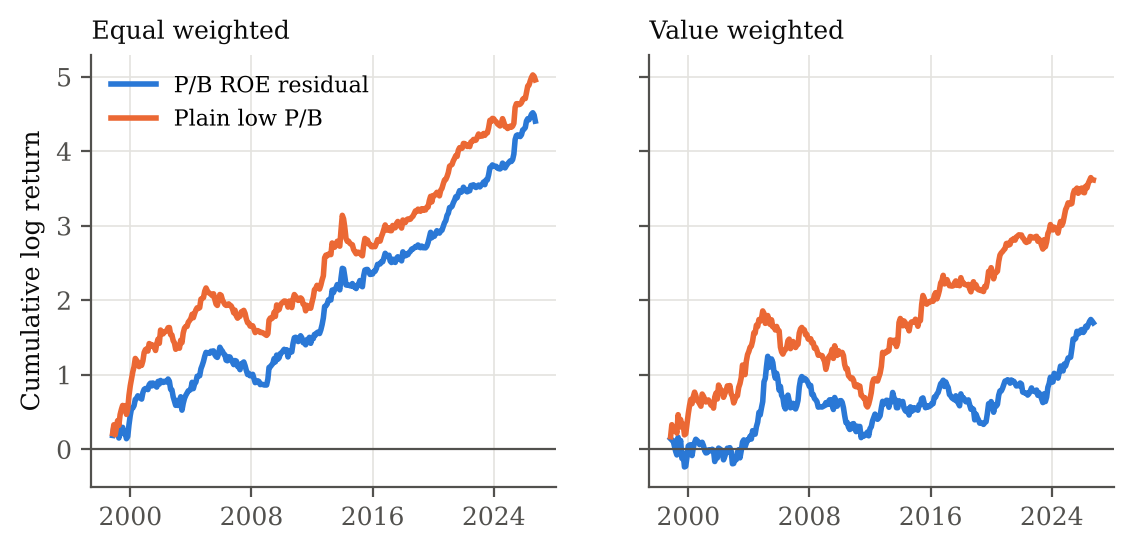
\includegraphics[width=0.92\textwidth]{fig3_cumulative_ls.png}
\caption{Cumulative log returns of the long short portfolios (cheapest minus dearest quintile).}
\label{fig:cumulative}
\end{figure}

\subsection{Risk adjustment}

Table~\ref{tab:ls} reports alphas. The equally weighted residual portfolio keeps a three factor alpha
of \FFew{}\% a month ($t = \FFewT{}$), but its loading on HML is \HMLew{}, confirming that it is
largely a value position. The value weighted alpha is \FFvw{}\% ($t = \FFvwT{}$). Plain value behaves
the same way. When the smallest 30\% of stocks by market capitalization are excluded each month, the
residual still earns \MicroLS{}\% a month before adjustment ($t = \MicroLST{}$), but its three factor
alpha falls to \MicroFF{}\% ($t = \MicroFFT{}$). The abnormal return lives among microcaps, which
are expensive and sometimes impossible to trade in size on the PSX.

\begin{table}[htbp]
\centering\footnotesize
\caption{Long short portfolios (cheapest minus dearest quintile). Mean and alphas are in percent per
month; $t$ statistics (Newey and West, six lags) in parentheses. Sharpe is annualized. 3F is the
three factor model with market, SMB and HML built from the same universe; HML $\beta$ is the loading
on HML in that model. ``No microcaps'' drops stocks below the 30th percentile of market cap each month.}
\label{tab:ls}
\setlength{\tabcolsep}{3pt}
\begin{tabular}{llrrrrrrrr}
\toprule
Signal & Weight & Mean & $t$ & Sharpe & CAPM $\alpha$ & $t$ & 3F $\alpha$ & $t$ & HML $\beta$ \\
\midrule
P/B ROE residual & EW & 1.46 & (4.70) & 0.96 & 1.36 & (4.75) & 0.90 & (3.73) & 0.62 \\
P/B ROE residual & VW & 0.75 & (1.83) & 0.37 & 0.46 & (1.22) & \ensuremath{-}0.02 & (\ensuremath{-}0.06) & 0.66 \\
Implied return $k$ & EW & 0.34 & (1.09) & 0.23 & 0.53 & (1.78) & 0.72 & (2.49) & 0.05 \\
Implied return $k$ & VW & 0.72 & (1.85) & 0.37 & 0.91 & (2.40) & 1.12 & (2.96) & \ensuremath{-}0.07 \\
Plain low P/B & EW & 1.67 & (4.54) & 0.96 & 1.43 & (4.32) & 0.78 & (3.08) & 0.81 \\
Plain low P/B & VW & 1.32 & (3.30) & 0.66 & 0.92 & (2.63) & 0.10 & (0.43) & 0.97 \\
ROE alone & EW & \ensuremath{-}0.48 & (\ensuremath{-}1.29) & \ensuremath{-}0.26 & \ensuremath{-}0.16 & (\ensuremath{-}0.46) & 0.47 & (1.56) & \ensuremath{-}0.44 \\
ROE alone & VW & 0.28 & (0.64) & 0.12 & 0.74 & (1.86) & 1.21 & (3.09) & \ensuremath{-}0.37 \\
P/B ROE residual, no microcaps & EW & 0.91 & (2.96) & 0.63 & 0.71 & (2.62) & 0.31 & (1.31) & 0.55 \\
P/B ROE residual, no microcaps & VW & 0.50 & (1.21) & 0.26 & 0.18 & (0.48) & \ensuremath{-}0.18 & (\ensuremath{-}0.50) & 0.53 \\
Plain low P/B, no microcaps & EW & 0.89 & (2.79) & 0.54 & 0.56 & (2.04) & 0.07 & (0.31) & 0.74 \\
Plain low P/B, no microcaps & VW & 0.96 & (2.60) & 0.50 & 0.53 & (1.73) & \ensuremath{-}0.04 & (\ensuremath{-}0.20) & 0.88 \\
\bottomrule
\end{tabular}

\end{table}

\subsection{Does ROE add anything to P/B?}

Table~\ref{tab:fm} answers H2 directly. On its own the cheapness score predicts returns strongly
(column 1), and it survives controls for size and momentum (column 2). Column 3 splits the model
into its parts: ln(B/P) predicts returns, while ROE does not (coefficient \FMthreeROE{}, $t =
\FMthreeROET{}$). In column 4, with both the residual and ln(B/P), neither is significant
(\FMfourResid{}, $t = \FMfourResidT{}$; and \FMfourVal{}, $t = \FMfourValT{}$): the two carry the
same information and the data cannot tell them apart. H2 is not supported. On the PSX, knowing a
firm's ROE does not help predict its return once its P/B is known.

\begin{table}[htbp]
\centering\small
\caption{Fama and MacBeth regressions of next month returns on standardized characteristics.
Coefficients are the average monthly slope in percent per one standard deviation; Newey and West
$t$ statistics in parentheses. All regressions include a constant (not shown).}
\label{tab:fm}
\begin{tabular}{lrrrr}
\toprule
 & (1) & (2) & (3) & (4) \\
\midrule
P/B ROE residual (cheapness) & 0.47 & 0.34 &  & 0.21 \\
 & (4.52) & (3.82) &  & (1.18) \\
ln(B/P) &  &  & 0.43 & 0.19 \\
 &  &  & (3.82) & (0.91) \\
ROE &  &  & 0.09 &  \\
 &  &  & (0.81) &  \\
ln(size) &  & \ensuremath{-}0.54 & \ensuremath{-}0.46 & \ensuremath{-}0.48 \\
 &  & (\ensuremath{-}4.26) & (\ensuremath{-}3.74) & (\ensuremath{-}3.71) \\
Momentum &  & 0.22 & 0.26 & 0.24 \\
 &  & (1.96) & (2.43) & (2.29) \\
\midrule
Months & 333 & 333 & 333 & 333 \\
\bottomrule
\end{tabular}

\end{table}

\subsection{The two period model}

The implied return $k$ of equation~(\ref{eq:implied}) adds ROE to the residual, so it tilts towards
profitable firms. Its raw equally weighted spread is small, \Kew{}\% a month ($t = \KewT{}$), because
the value and profitability parts partly offset each other. After the factor adjustment, however, the
value weighted implied return portfolio earns \Kvwff{}\% a month ($t = \KvwffT{}$), with no HML
loading. This alpha comes from profitability: sorting on ROE alone gives a similar value weighted
three factor alpha of \ROEvwff{}\% ($t = \ROEvwffT{}$). This is the profitability premium documented
by \citet{famafrench2006}, appearing here among larger PSX firms. The two period model does capture
something different from value, but what it captures is profitability, not convergence of P/B to the
line.

\subsection{Sectors}

Table~\ref{tab:sectors} runs the model within the three largest sectors. In textiles the within
sector residual works well: the tercile long short portfolio earns \TEXew{}\% a month ($t =
\TEXewT{}$), the three factor alpha is \TEXff{}\% ($t = \TEXffT{}$), and the rank IC is about twice
the whole market figure. In banks (\BANKew{}\%, $t = \BANKewT{}$) and cement (\CEMew{}\%, $t =
\CEMewT{}$) the spreads are smaller and not significant, and the three factor alphas are close to zero. H3 holds only
for textiles. One explanation is that textiles is a large group of small, homogeneous, export
oriented firms whose prices react slowly, while banks and cement are few, large and widely followed.
With 16 to 20 firms a month, though, the bank and cement tests have little power.

\begin{table}[htbp]
\centering\small
\caption{Within sector tests. Residuals come from a separate regression of ln(P/B) on ROE inside each
sector each month; portfolios are terciles. Firms is the average number of firms per month. LS mean
and 3F $\alpha$ in percent per month. Rank IC is the average monthly Spearman correlation between
the cheapness score and next month return.}
\label{tab:sectors}
\begin{tabular}{llrrrrrrr}
\toprule
Sector & Weight & Firms & LS mean & $t$ & 3F $\alpha$ & $t$ & Rank IC & $t$ \\
\midrule
Banks & EW & 20 & 0.55 & (1.44) & 0.05 & (0.14) & \ensuremath{-}0.001 & (\ensuremath{-}0.07) \\
 & VW & 20 & 0.31 & (0.87) & \ensuremath{-}0.07 & (\ensuremath{-}0.20) &  &  \\
Cement & EW & 16 & 0.86 & (1.72) & \ensuremath{-}0.27 & (\ensuremath{-}0.64) & \ensuremath{-}0.025 & (\ensuremath{-}1.41) \\
 & VW & 16 & 0.91 & (1.57) & \ensuremath{-}0.01 & (\ensuremath{-}0.04) &  &  \\
Textiles & EW & 49 & 1.42 & (3.58) & 0.97 & (2.57) & 0.042 & (3.62) \\
 & VW & 49 & 1.43 & (2.77) & 0.85 & (1.80) &  &  \\
\midrule
Whole market & EW & & & & & & 0.021 & (2.86) \\
\bottomrule
\end{tabular}

\end{table}

\subsection{Hit rates and the chance rate}

Table~\ref{tab:hits} reports the model's ``accuracy'', the share of stocks for which the cheap label
matches outperformance. Monthly, the hit rate for the whole market is \HitM\%, against a chance rate
of \BaseM\% from equation~(\ref{eq:chance}). Over 12 months from each October it is \HitA\% against
\BaseA\% ($t = \HitAT{}$). Hit rates in the low to mid fifties are therefore weak evidence by
themselves: a modest excess over the chance rate is consistent with the long short returns above,
but a hit rate should never be read against 50\%. A strategy can earn high long short returns with a
hit rate near chance if it is right about the few stocks that move most, which is the pattern in
Figure~\ref{fig:quintiles}.

\begin{table}[htbp]
\centering\small
\caption{Hit rates. A hit is a stock labelled cheap (negative residual) that beats the cross
sectional average return, or one labelled dear that does not. The chance rate is equation
(\ref{eq:chance}). Excess is the average of hit rate minus chance rate, in percentage points; $t$
statistics in parentheses. The 12 month test forms signals at the end of each October.}
\label{tab:hits}
\begin{tabular}{llrrrrr}
\toprule
Sample & Horizon & Periods & Hit rate (\%) & Chance rate (\%) & Excess & $t$ \\
\midrule
Market & 1 month & 334 & 50.1 & 49.6 & 0.48 & (1.72) \\
Banks & 1 month & 256 & 49.8 & 50.1 & \ensuremath{-}0.28 & (\ensuremath{-}0.39) \\
Cement & 1 month & 249 & 48.7 & 50.3 & \ensuremath{-}1.60 & (\ensuremath{-}2.04) \\
Textiles & 1 month & 267 & 50.2 & 49.3 & 0.89 & (1.60) \\
Market & 12 months (Oct) & 28 & 51.5 & 49.0 & 2.49 & (2.44) \\
Banks & 12 months (Oct) & 20 & 53.3 & 50.0 & 3.32 & (1.22) \\
Cement & 12 months (Oct) & 20 & 49.7 & 50.4 & \ensuremath{-}0.69 & (\ensuremath{-}0.24) \\
Textiles & 12 months (Oct) & 21 & 50.0 & 48.1 & 1.90 & (1.43) \\
\bottomrule
\end{tabular}

\end{table}

\subsection{Robustness}

\paragraph{Subperiods.} Table~\ref{tab:sub} splits the sample into three periods. The equally weighted
residual spread is positive in all three and significant in the last two; the value weighted spread
is never significant. Plain value is about as strong with equal weights and stronger with value weights in every period. No year is dropped from any
test, including the 2008 crisis, when the exchange imposed a price floor for several months, and the
2020 pandemic.

\begin{table}[htbp]
\centering\small
\caption{Long short returns by subperiod, percent per month, Newey and West $t$ statistics in
parentheses.}
\label{tab:sub}
\begin{tabular}{llrrrrrr}
\toprule
Signal & Weight & \multicolumn{2}{c}{1998 to 2007} & \multicolumn{2}{c}{2008 to 2016} & \multicolumn{2}{c}{2017 to 2026} \\
\midrule
P/B ROE residual & EW & 1.09 & (1.67) & 1.65 & (3.18) & 1.64 & (4.14) \\
P/B ROE residual & VW & 1.17 & (1.28) & 0.23 & (0.42) & 0.84 & (1.42) \\
Plain low P/B & EW & 1.74 & (2.19) & 1.42 & (2.14) & 1.82 & (4.69) \\
Plain low P/B & VW & 1.68 & (2.08) & 0.98 & (1.27) & 1.30 & (2.86) \\
Textiles, within sector & EW & 1.26 & (1.08) & 1.94 & (2.87) & 0.99 & (2.07) \\
Textiles, within sector & VW & 1.72 & (1.49) & 2.06 & (2.16) & 0.78 & (1.25) \\
\bottomrule
\end{tabular}

\end{table}

\paragraph{Trading costs.} The residual portfolio replaces about \Turn\% of its long and short
holdings each month. Table~\ref{tab:costs} subtracts one way costs of 50 and 100 basis points per
trade. With monthly rebalancing the residual spread is still \NetHundred{}\% a month at 100 basis
points ($t = \NetHundredT{}$); rebalancing once a year in October loses some gross return but saves
most of the cost. The textile strategy is more fragile: its annual version earns much less, which
suggests that the within sector mispricing it trades is corrected within a few months. Short sales
are restricted and costly on the PSX, so the long leg matters most in practice: the cheapest
quintile beats the equally weighted market by \TopEx\% a month ($t = \TopExT{}$), but only with equal weights.

\begin{table}[htbp]
\centering\small
\caption{Net long short returns after trading costs, percent per month, Newey and West $t$ statistics
in parentheses. Costs are one way, charged on each name bought or sold. Annual portfolios are formed
at the end of October and held for twelve months.}
\label{tab:costs}
\begin{tabular}{llrrrrrr}
\toprule
Signal & Rebalancing & \multicolumn{2}{c}{0 bps} & \multicolumn{2}{c}{50 bps} & \multicolumn{2}{c}{100 bps} \\
\midrule
P/B ROE residual & monthly & 1.46 & (4.70) & 1.13 & (3.65) & 0.79 & (2.57) \\
P/B ROE residual & annual (Oct) & 1.22 & (3.86) & 1.05 & (3.36) & 0.89 & (2.84) \\
Textiles, within sector & monthly & 1.42 & (3.58) & 1.02 & (2.61) & 0.62 & (1.61) \\
Textiles, within sector & annual (Oct) & 0.55 & (1.21) & 0.38 & (0.84) & 0.22 & (0.47) \\
Implied return $k$ (two period) & monthly & 0.34 & (1.09) & 0.03 & (0.10) & \ensuremath{-}0.28 & (\ensuremath{-}0.90) \\
Implied return $k$ (two period) & annual (Oct) & 0.07 & (0.23) & \ensuremath{-}0.10 & (\ensuremath{-}0.35) & \ensuremath{-}0.27 & (\ensuremath{-}0.94) \\
\bottomrule
\end{tabular}

\end{table}


\section{Discussion and limitations}\label{sec:discussion}

The results fit a familiar pattern in the anomaly literature. \citet{famafrench2008} and
\citet{houxuezhang2020} show that many return anomalies are strongest, or exist only, among microcaps,
and \citet{rouwenhorst1999} and \citet{asnessmoskowitzpedersen2013} document a value premium across
emerging and developed markets. The P/B ROE residual on the PSX looks like one more expression of the
value premium, with most of its abnormal return in the smallest and least liquid stocks.

Several limitations deserve mention. Compustat Global does not report delisting returns, so the
last return of a firm that delists is missing rather than, say, a large loss; because cheap firms
are more likely to fail, this may overstate the long leg. The factor models use factors built from
the same small universe, which are noisier than the standard factors available for the United States.
The early years have fewer than 100 firms a month. Many tests are reported, and with this many
specifications some $t$ statistics above two are expected by chance; the conclusions above rest on
the patterns that hold across specifications rather than on any single number. Finally, the model's
linear form is an approximation; a richer specification with growth and payout, as in
equation~(\ref{eq:gordon}), might do better within sectors.

\section{Conclusion}\label{sec:conclusion}

The P/B ROE model describes how the PSX prices stocks well: across firms, ROE explains a large and
stable part of the variation in P/B. As a trading rule it works, but mostly for a reason other than
the one it advertises. Stocks far below the P/B ROE line earn high returns, but they earn them because
they are cheap, not because they are cheap given their profitability, and the abnormal part of the
return is concentrated in microcaps. The forward looking two period form of the model picks up the
profitability premium among larger firms instead. Within sectors, the model is useful in textiles and
not in banks or cement. For an investor on the PSX, the practical lesson is that a value tilt
captures most of what the model offers, and that claims of high accuracy should always be compared
with the rate a random guess would achieve.

\bibliographystyle{plainnat}
\begin{thebibliography}{99}
\setlength{\itemsep}{2pt}

\bibitem[Asness, Moskowitz and Pedersen(2013)]{asnessmoskowitzpedersen2013}
Asness, C.~S., Moskowitz, T.~J. and Pedersen, L.~H. (2013). Value and momentum everywhere.
\textit{Journal of Finance}, 68(3), 929--985.

\bibitem[Fama and French(1993)]{famafrench1993}
Fama, E.~F. and French, K.~R. (1993). Common risk factors in the returns on stocks and bonds.
\textit{Journal of Financial Economics}, 33(1), 3--56.

\bibitem[Fama and French(2006)]{famafrench2006}
Fama, E.~F. and French, K.~R. (2006). Profitability, investment and average returns.
\textit{Journal of Financial Economics}, 82(3), 491--518.

\bibitem[Fama and French(2008)]{famafrench2008}
Fama, E.~F. and French, K.~R. (2008). Dissecting anomalies. \textit{Journal of Finance}, 63(4),
1653--1678.

\bibitem[Fama and MacBeth(1973)]{famamacbeth1973}
Fama, E.~F. and MacBeth, J.~D. (1973). Risk, return, and equilibrium: Empirical tests.
\textit{Journal of Political Economy}, 81(3), 607--636.

\bibitem[Hou, Xue and Zhang(2020)]{houxuezhang2020}
Hou, K., Xue, C. and Zhang, L. (2020). Replicating anomalies. \textit{Review of Financial Studies},
33(5), 2019--2133.

\bibitem[Ince and Porter(2006)]{inceporter2006}
Ince, O.~S. and Porter, R.~B. (2006). Individual equity return data from Thomson Datastream: Handle
with care! \textit{Journal of Financial Research}, 29(4), 463--479.

\bibitem[Newey and West(1987)]{neweywest1987}
Newey, W.~K. and West, K.~D. (1987). A simple, positive semi\mbox{-}definite, heteroskedasticity and
autocorrelation consistent covariance matrix. \textit{Econometrica}, 55(3), 703--708.

\bibitem[Ohlson(1995)]{ohlson1995}
Ohlson, J.~A. (1995). Earnings, book values, and dividends in equity valuation.
\textit{Contemporary Accounting Research}, 11(2), 661--687.

\bibitem[Rouwenhorst(1999)]{rouwenhorst1999}
Rouwenhorst, K.~G. (1999). Local return factors and turnover in emerging stock markets.
\textit{Journal of Finance}, 54(4), 1439--1464.

\bibitem[Wilcox(1984)]{wilcox1984}
Wilcox, J.~W. (1984). The P/B\mbox{-}ROE valuation model. \textit{Financial Analysts Journal},
40(1), 58--66.

\bibitem[Wilcox and Philips(2005)]{wilcoxphilips2005}
Wilcox, J.~W. and Philips, T.~K. (2005). The P/B\mbox{-}ROE valuation model revisited.
\textit{Journal of Portfolio Management}, 31(4), 56--66.

\end{thebibliography}

\appendix
\section{Variable definitions}

\begin{tabular}{p{0.22\textwidth}p{0.7\textwidth}}
\toprule
Variable & Definition (Compustat Global item) \\
\midrule
Book equity & Common equity \texttt{ceq}; total equity \texttt{seq} if \texttt{ceq} is missing \\
ROE & Income before extraordinary items \texttt{ib} over book equity at the start of the fiscal year \\
Market cap & Month end price \texttt{prccd} times shares outstanding \texttt{cshoc} \\
P/B & Market cap over the latest public book equity \\
Return & Change in \texttt{prccd}/\texttt{ajexdi}$\times$\texttt{trfd} (includes dividends) \\
Days traded & Days in the month with positive volume \texttt{cshtrd} \\
Momentum & Compounded return over months $t-11$ to $t-1$ \\
Public date & Fiscal year end plus four months; used for at most 14 further months \\
\bottomrule
\end{tabular}

\end{document}
